% Moved to section 1.4 Definitions, acronyms, abbreviations


\begin{table}[H]
    \centering
    \begin{tabular}{|l|p{0.75\textwidth}|}
        \hline % ---------------------------------------------------------------------
    	\textsc{id}                 &   PM.1\\
    	\hline % ---------------------------------------------------------------------
    	\textsc{Name}               &   Visualize the performance data of each farmer\\
    	\hline % ---------------------------------------------------------------------
    	\textsc{Actor}             &   Policy maker\\
    	\hline % ---------------------------------------------------------------------
    	\textsc{Entry condition}   &   Policy maker has logged in\\
    	\hline % ---------------------------------------------------------------------
    	\textsc{Events flow}         &   %\footnotesize
            	                        \begin{itemize}
                                    	    \item Policy maker goes to the “Farmer’s performance” section
                                    	    \item The system displays options to let user select filters about weather type, product type
                                    		\item Policy maker selects desired filters
                                    		\item The system displays the list of farmers divided by performance
                                    		\item Policy maker selects interested farmer’s name
                                    		\item The system shows detailed information about that farmer’s production
                                        \end{itemize}\\
        \hline % ---------------------------------------------------------------------
        \textsc{Exit condition}    &  The system returns to the main page of policy maker\\
    	\hline % ---------------------------------------------------------------------
    	\textsc{Output}             &  \begin{itemize}
    	    \item Policy maker has obtained the farmer's production data they were looking for
    	\end{itemize}\\
    	\hline % ---------------------------------------------------------------------
    	\textsc{Exception}         &  Policy maker could not find the name of farmer who should exist. The system displays an error message\\
    	\hline % ---------------------------------------------------------------------
        
    \end{tabular}
    \caption{\label{tab:visualize_farmer_performance}Visualize the performance data of farmers} 
\end{table}

\begin{figure}[H]
    \centering
    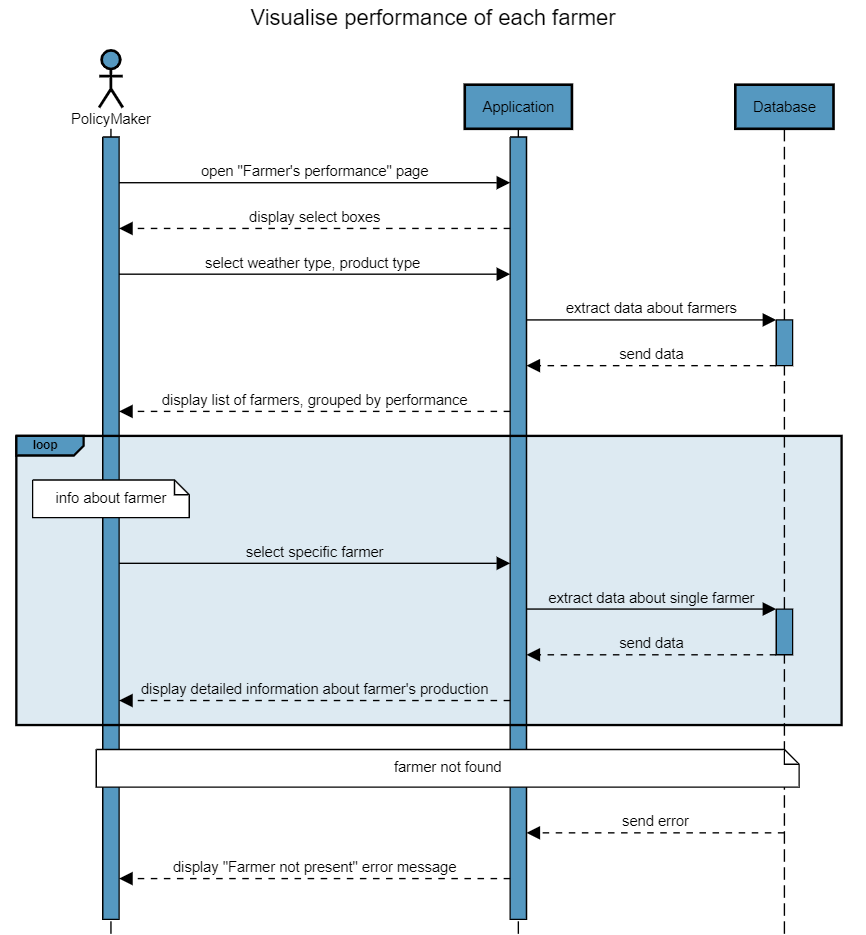
\includegraphics[scale=0.5]{Images/Sequence diagrams/SE2 - visualize performance (pm).png}
    \caption{Visualize the performance data of farmers - sequence diagram}
    \label{fig:seq_diag_visualize_performance}
\end{figure}

\begin{table}[H]
    \centering
    \begin{tabular}{|l|p{0.75\textwidth}|}
        \hline % ---------------------------------------------------------------------
    	\textsc{id}                 &   PM.2\\
    	\hline % ---------------------------------------------------------------------
    	\textsc{Name}               &   Manage the incentives of high performing farmers \\
    	\hline % ---------------------------------------------------------------------
    	\textsc{Actor}             &   Policy maker\\
    	\hline % ---------------------------------------------------------------------
    	\textsc{Entry condition}   &   Policy maker has logged in\\
    	\hline % ---------------------------------------------------------------------
    	\textsc{Events flow}         &   %\footnotesize
            	                        \begin{itemize}
                                    	    \item Policy maker goes to the “Farmer’s performance” section
                                    		\item The system displays a page with the list of farmers (grouped by performance) and a column which clarifies the status of their incentives 
                                       		\item Policy maker selects the interested farmer’s incentive column
                                    		\item The system shows detailed information about farmer’s incentives status
                                    		\item Policy maker clicks "Select incentive" button
                                    		\item The system shows the possible choices
                                    		\item Policy maker selects the incentive to give
                                    		\item The system shows the popup to ask a confirmation to proceed
                                    		\item Policy maker clicks "Confirm" button
                                    		\item The system shows the updated incentive column
                                        \end{itemize}\\
        \hline % ---------------------------------------------------------------------
        \textsc{Exit condition}    &  The system returns to the main page of policy maker\\
    	\hline % ---------------------------------------------------------------------
    	\textsc{Output}             &  \begin{itemize}
    	    \item Policy maker has managed the incentive to give
    	    \item The farmer correctly received the inventive
    	\end{itemize}\\
    	\hline % ---------------------------------------------------------------------
    	\textsc{Exception}         &  Policy maker wrongly selects an incentive data. The 
    	system shows a popup to ask a confirmation to proceed. The policy maker can redo the operation by clicking on “Cancel” button\\
    	\hline % ---------------------------------------------------------------------
        
    \end{tabular}
    \caption{\label{tab:visualize_incentives}Manage the incentives of farmers} 
\end{table}

\begin{figure}[H]
    \centering
    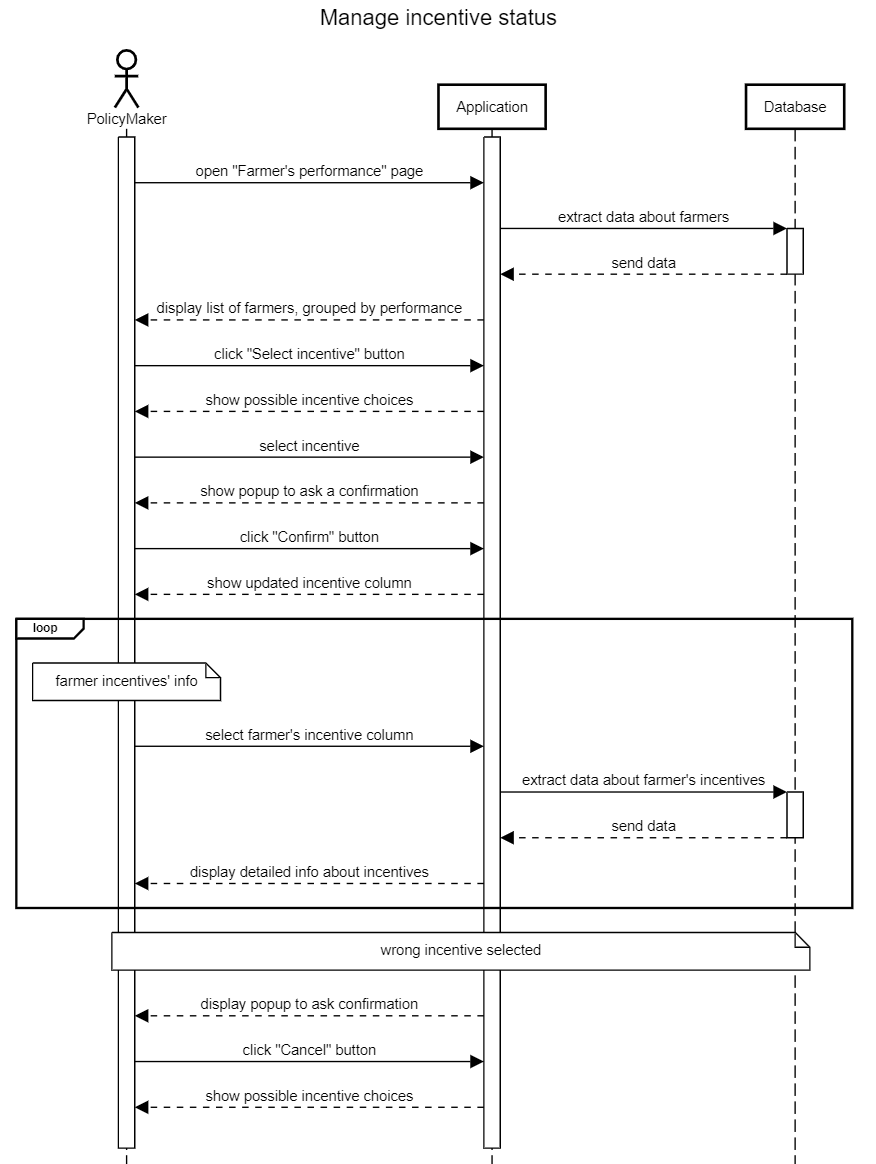
\includegraphics[scale=0.5]{Images/Sequence diagrams/SE2 - manage incentive status (pm).png}
    \caption{Manage the incentives of farmers - sequence diagram}
    \label{fig:seq_diag_visualize_incentive}
\end{figure}

\begin{table}[H]
    \centering
    \begin{tabular}{|l|p{0.75\textwidth}|}
        \hline % ---------------------------------------------------------------------
    	\textsc{id}                 &   PM.3\\
    	\hline % ---------------------------------------------------------------------
    	\textsc{Name}               &   Visualize the effectiveness of the steering initiatives\\
    	\hline % ---------------------------------------------------------------------
    	\textsc{Actor}             &   Policy maker\\
    	\hline % ---------------------------------------------------------------------
    	\textsc{Entry condition}   &   Policy maker has logged in\\
    	\hline % ---------------------------------------------------------------------
    	\textsc{Events flow}         &   %\footnotesize
            	                        \begin{itemize}
                                    	    \item Policy maker goes to the “Effectiveness of initiatives” section
                                    	    \item The system displays options to let user select filters about weather type, product type
                                    		\item Policy maker selects the desired filters
                                    		\item The system displays a page with categorized farmers, highlighting those who have improved their performance significantly within a year
                                    		\item Policy maker selects interested farmer’s name
                                    		\item The system shows detailed information about the farmer’s performance trend, the problems encountered, the history of requests and visits
                                        \end{itemize}\\
        \hline % ---------------------------------------------------------------------
        \textsc{Exit conditions}    &  The system returns to the main page of policy maker\\
    	\hline % ---------------------------------------------------------------------
    	\textsc{Output}             &  \begin{itemize}
    	    \item Policy maker has obtained the history of performance data and interaction between farmers and agronomists they were looking for
    	\end{itemize}\\
    	\hline % ---------------------------------------------------------------------
    	\textsc{Exception}         &  Policy maker couldn’t find the name of farmer who should exist. The system displays an error message\\
    	\hline % ---------------------------------------------------------------------
        
    \end{tabular}
    \caption{\label{tab:visualize_iprovement}Visualize the effectiveness of the steering initiatives}
\end{table}

\begin{figure}[H]
    \centering
    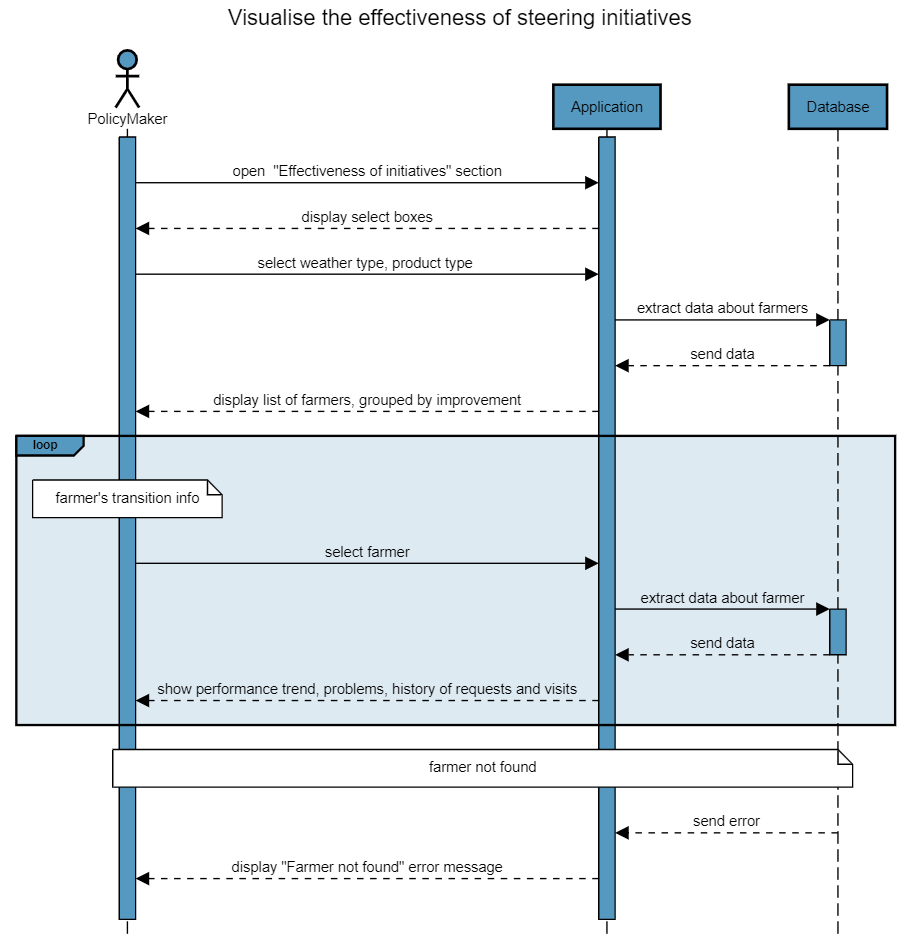
\includegraphics[scale=0.5]{Images/Sequence diagrams/SE2 - visualise effectiveness of steering initiatives (pm).png}
    \caption{Visualize the effectiveness of the steering initiatives - sequence diagram}
    \label{fig:fig:seq_diag_visualize_improvement}
\end{figure}

\begin{table}[H]
    \centering
    \begin{tabular}{|l|p{0.75\textwidth}|}
        \hline % ---------------------------------------------------------------------
    	\textsc{id}                 &   PM.4\\
    	\hline % ---------------------------------------------------------------------
    	\textsc{Name}               &   Ask high performing farmers to write good practices\\
    	\hline % ---------------------------------------------------------------------
    	\textsc{Actor}             &   Policy maker\\
    	\hline % ---------------------------------------------------------------------
    	\textsc{Entry condition}   &   Policy maker has logged in\\
    	\hline % ---------------------------------------------------------------------
    	\textsc{Events flow}         &   %\footnotesize
            	                        \begin{itemize}
                                    	    \item Policy maker goes to the “Farmer’s performance” section
                                    		\item The system displays a page with the list of farmers grouped by performance
                                    		\item Policy maker selects interested high performing farmer’s name
                                    		\item The system shows the detailed information about farmer’s production and "request writing" button
                                    		\item Policy maker clicks "Request writing" button
                                    		\item The system shows a popup to ask the confirmation to proceed
                                    		\item Policy maker clicks "Confirm" button
                                    		\item The system sends the request to the selected farmer and shows a message to notify the success of the operation
                                        \end{itemize}\\
        \hline % ---------------------------------------------------------------------
        \textsc{Exit condition}    &  The system returns to the Farmer’s performance page\\
    	\hline % ---------------------------------------------------------------------
    	\textsc{Output}             &  \begin{itemize}
    	    \item Policy maker has requested the high performing farmer to write their good practice
    	    \item Farmer has received the good practice request
    	\end{itemize}\\
    	\hline % ---------------------------------------------------------------------
    	\textsc{Exception}         &  Policy maker wrongly selects a farmer. The 
    	system shows a popup to ask a confirmation to proceed. The policy maker can redo the operation by clicking on “Cancel” button\\
    	\hline % ---------------------------------------------------------------------
        
    \end{tabular}
    \caption{\label{tab:visualize_iprovement}Ask a farmer to write good practices} 
\end{table}

\begin{figure}[H]
    \centering
    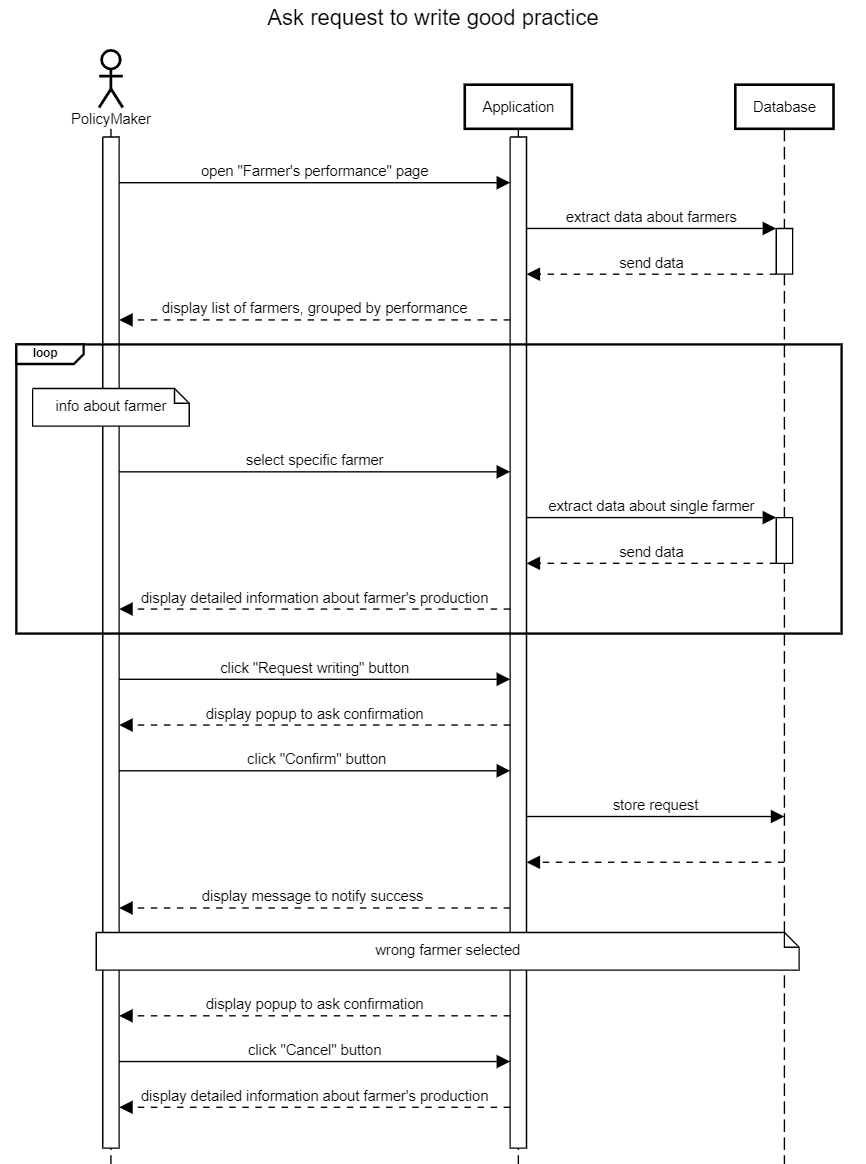
\includegraphics[scale=0.5]{Images/Sequence diagrams/SE2 - Ask request to write good practice (pm).png}
    \caption{Ask request to write good practice - sequence diagram}
    \label{fig:my_label}
\end{figure}

